\begin{enumerate}[label=\thesection.\arabic*.,ref=\thesection.\theenumi]
\numberwithin{equation}{enumi}

\begin{abstract}
This document contains the solution to a Gradient decent question.\\
\end{abstract}
Download all python codes from 
%
\begin{lstlisting}
https://github.com/Jayanth9969/EE5600/blob/master/Assignment4/code.py
\end{lstlisting}

\section{Problem}
    Find the maximum and minimum values, if any of the following function \\
    $f(x) = -(x-1)^2+10$ \\ \\
    
\section{Solution}

    Given $f(x) = -(x-1)^2+10$ \\
    % \boldsymbol{Claim}: f(x) is Convex \\
    % \boldsymbol{Proof}:\\
    % First we prove f(x) is convex.\\
    A function is said to be convex if following inequality is true:
    \begin{align}
        \lambda f(x_1)+(1-\lambda) f(x_2) \geq f(\lambda x_1+(1-\lambda) x_2
    \end{align}
    % and for $\lambda$ \in [0,1] \space and \space $x_1,x_2$ \in domain \space of \space f(x)\\  
    
    or we can check that is f''(x)) $>$ 0 then the function is convex else the function will be concave  \\
    
    \begin{align}
        f(x) = -(x-1)^2+10 \\
        f'(x) = -2(x-1) \\
        f''(x) = -2 
    \end{align}
    
    Since $f''(x) < 0$ so f(x) is concave function.So we can find the maximum using gradient ascent method.Since function is concave it has only maximum and minimum will be -infinity \\
    
    % Solution using gradient ascent method is available at:
    % \begin{lstlisting}
    % https://github.com/Jayanth9969/EE5600/blob/master/Assignment4/code.py
    % \end{lstlisting}
    
    we can also find the maximum as following, Since derivative of f(x) at maximum is zero.
    \begin{align}
        f'(x) &= -2(x-1) \\
        0 &= -2(x-1) \\
        x &= 1
    \end{align}
    
    Thus maximum occurs at x = 1 \\
    \begin{align}
        x = 1 \\
        f(x) = -(x-1)^2+10 \\
        f(1) = -(1-1)^2+10 \\
        f(1) = 10
    \end{align}
    Thus maximum attainable value of f(x) is 10 at x = 1 
    \begin{figure}[h]
    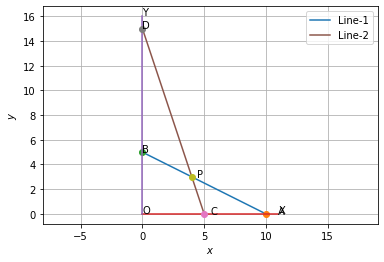
\includegraphics[width=\columnwidth]{Figure_1.png}
    \caption{Here B is maximum point and A is intial answer in gradient ascent method}
    \end{figure}\\

    
    % \begin{align}
    %     \lambda f(x_1)+(1-\lambda) f(x_2) \geq f(\lambda x_1 + (1-\lambda) x_2 \\
    %     \lambda (-(x_1-1)^2+10) + (1-\lambda)(-(x_2-1)^2+10) \geq -(\lambda x_1 + (1-\lambda)(x_2-1))^2+10 \\
    %     -\lambda (x_1-1)^2 + 10\lambda - (x_2-1)^2 + 10 + \lambda (x_2-1)^2  -10\lambda \geq -(\lambda (x_1-1)^2 + (1-\lambda)(x_2-1))^2 + 10 \\
    %     -\lambda (x_1-1)^2 - (x_2-1)^2 + \lambda (x_2-1)^2 &\geq -(\lambda^2 (x_1-1)^2 + (1-\lambda)^2 (x_2-1)^2 + 2\lambda(1-\lambda)(x_1-1)(x_2-1) \\
    %     -\lambda (x_1-1)^2 - (x_2-1)^2 + \lambda (x_2-1)^2 \geq -(x_1-1)^2(-\lambda^2+\lambda)-(x_2-1)^2(-\lambda^2+\lambda)-2\lambda(1-\lambda)(x_1-1)(x_2-1) \\
    %     0 \geq (\lambda^2-\lambda)((x_1-1)^2+(x_2-1)^2+2\lambda(1-\lambda)(x_1-1)(x_2-1) \\
    %     0 \geq \lamda(1-\lamda)((x_1-1)-(x_2-1))^2 \\
    % \end{align}
    
    % The above inequality is not true for all values from domain.
    % Hence the given function f(x) is concave.So we gonna use gradient ascent to find the maximum value.\\
    The solution can found using gradient ascent method is as follows: \\
    Let us Suppose at x = -5 (initial guess)be point where maximum value was attained,thus $x_0 = -5$.
    Our Update Equation will be: 
    \begin{align}
        x_1 &= x_0 + f'(x_0) \times rate \\
        error &= \lvert (x_0 - x_1) \rvert\\
        x_0 &= x_1 
    \end{align}
    Here, rate = 0.1 \\
    we do update our $x_0$ until error between $x_0$ and $x_1$ becomes less than 0.000000001. \\
    In this case using code.py ,we got answer after 95 iterations.we got maximum value  attained is 10.0 occured at x = 0.9999999962700757 .
    
    
\end{enumerate}